\section{Introducción}
Un proceso se define como un programa en ejecución dentro de un sistema operativo. Los procesos conforman la mayoría de las acciones que se realizan dentro de un sistema operativo, desde la las entradas y salidas del mismo, la creación o eliminación de archivos y carpetas, hasta la ejecución de programas más complejos.

Inicialmente dentro del mundo de la computación los sistemas operativos trabajaban un proceso después de otro de manera secuencial, es decir, un proceso debía terminar por completo para que el siguiente empezara a ejecutarse. Sin embargo, posteriormente se avanzó en este sentido consiguiendo que los sistemas operativos trabajen los procesos en paralelo, esto quiere decir que la CPU (Unidad central de procesamiento) atiende a varios procesos al mismo tiempo.

<<\textit{Todas las computadoras modernas pueden hacer varias cosas al mismo tiempo. Mientras ejecuta un programa de usuario, una computadora también puede estar leyendo de un disco y enviando texto a una pantalla o impresora. En un sistema de multiprogramación, la CPU también conmuta de un programa a otro, ejecutando cada uno durante decenas o centenas de milisegundos. Si bien, estrictamente hablando, en un instante dado la CPU está ejecutando sólo un programa, en el curso de un segundo puede trabajar con varios programas, dando a los usuarios la ilusión de paralelismo.}>> \parencite{tanenbaum1997sistemas}. En este sentido, los sistemas operativos trabajan procesos en paralelo, pero en una CPU única tal como se ilustra en la figura~\ref{fig:procesosParalelos}.

\begin{figure}[!ht]
    \centering
    \caption{Procesos en paralelo}
    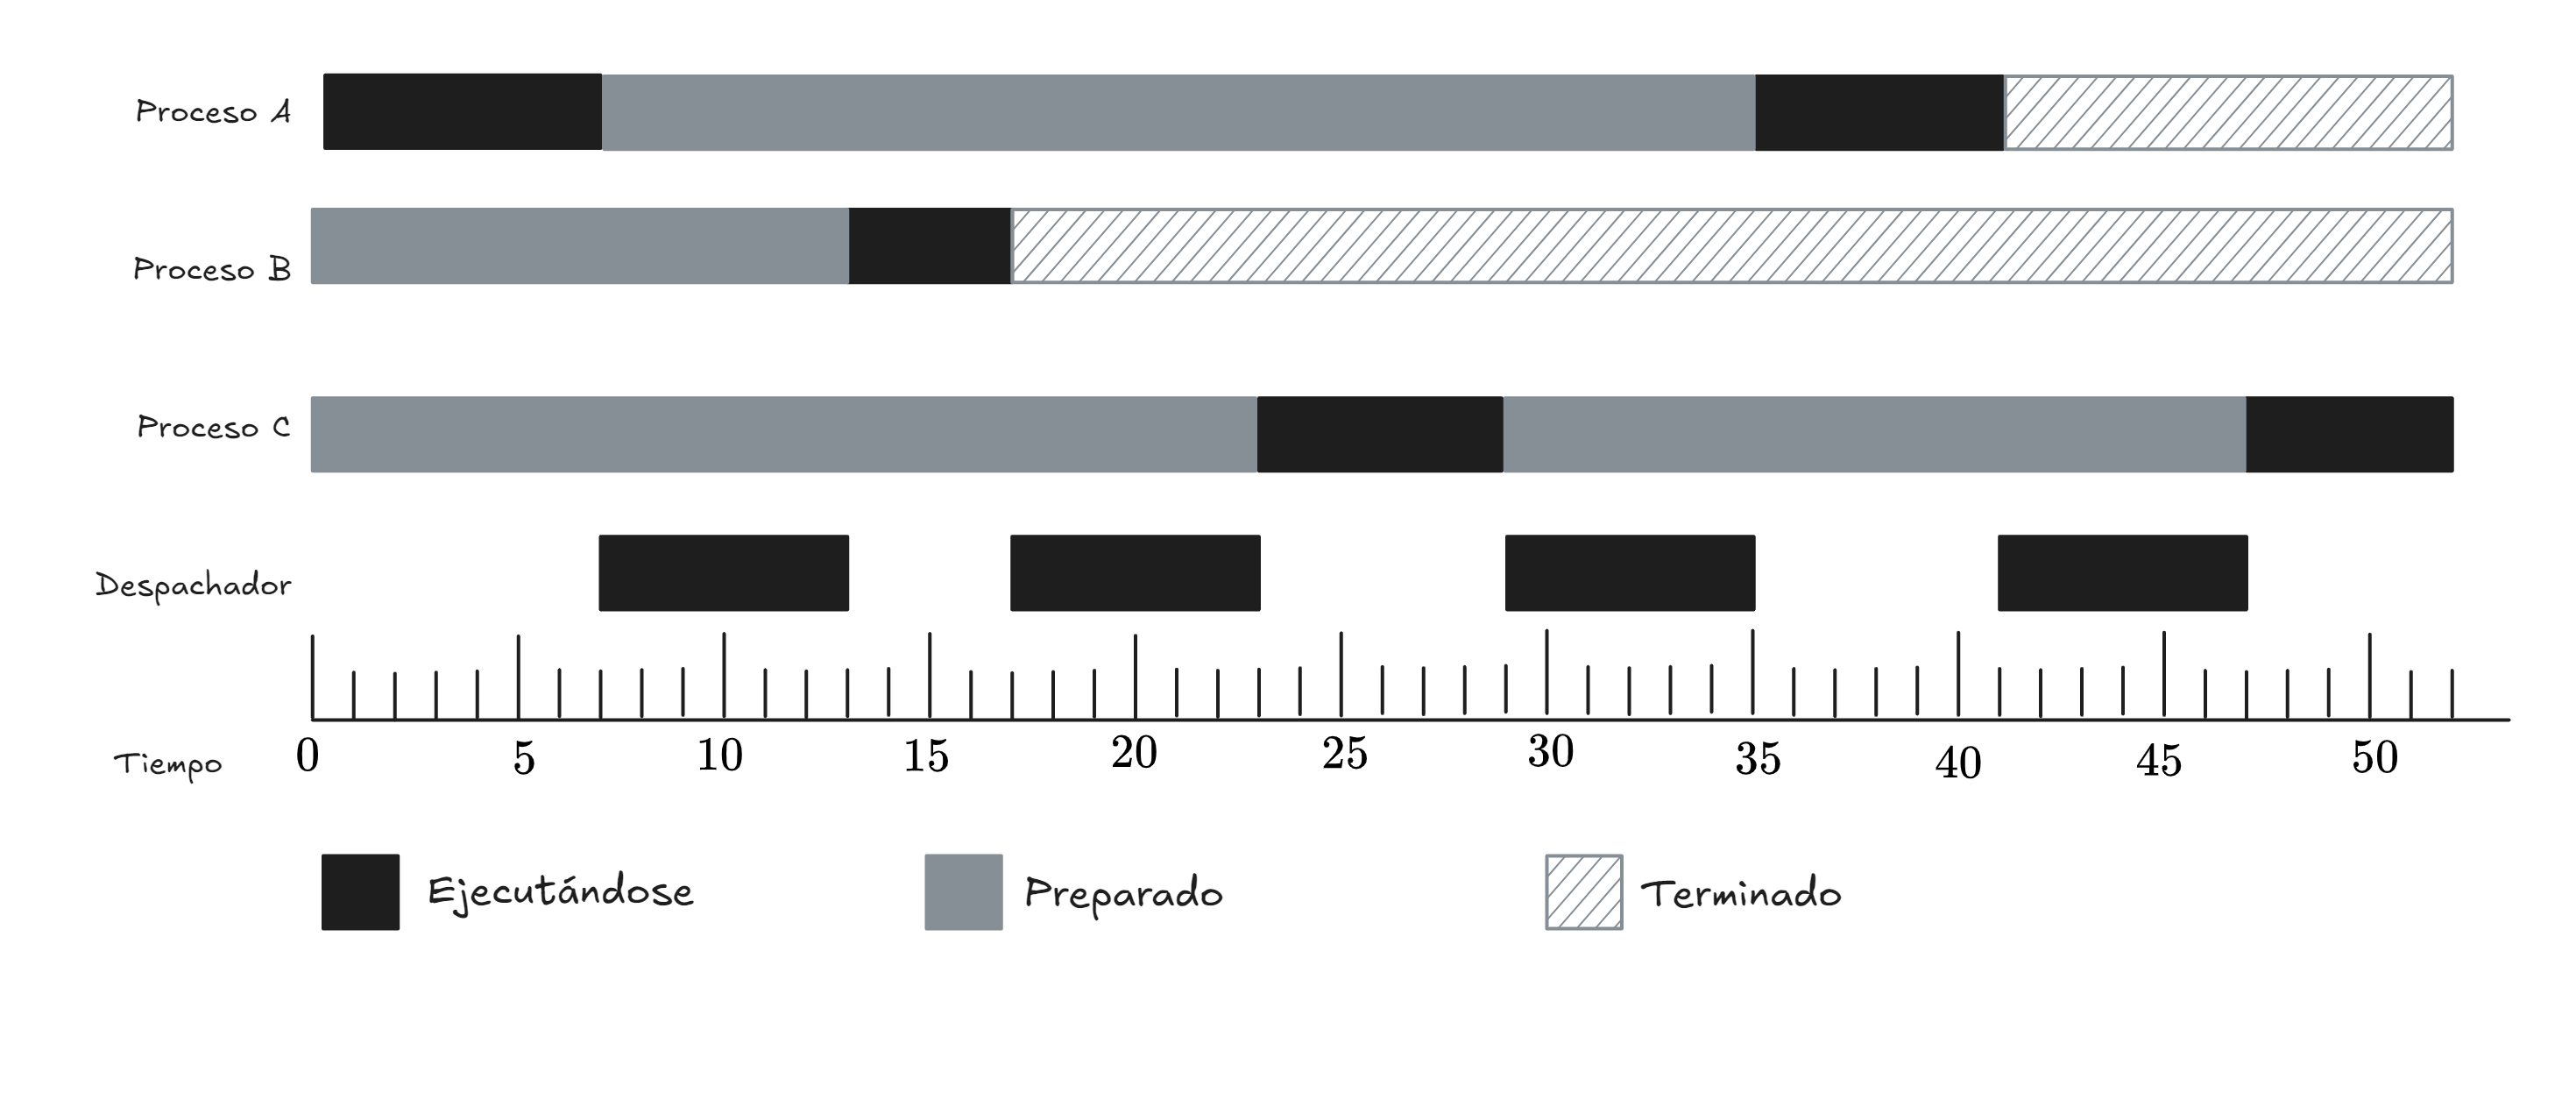
\includegraphics[width=0.7\textwidth]{src/images/Procesos en paralelo.png}\label{fig:procesosParalelos}
\end{figure}

Esto ocasiona que al querer trabajar con procesos de manera paralela (Por ejemplo, dejar un proceso en segundo plano) sea necesario tener en cuenta este comportamiento.

Adicionalmente, para la compresión del funcionamiento de procesos dentro de un sistema operativo, es necesario poder hacer experimentos con los mismos, lo que se hará en el presente laboratorio mediante el uso de procesos productores (generadores de información) y temporizadores que nos permitirán comprender su funcionamiento y tiempos de acción.
